
%(BEGIN_QUESTION)
% Copyright 2008, Tony R. Kuphaldt, released under the Creative Commons Attribution License (v 1.0)
% This means you may do almost anything with this work of mine, so long as you give me proper credit

The amount of voltage between two different ``hot'' conductors of a Y-type three-phase AC power system may be represented in the form of a vector diagram, where the lengths of lines represent voltage magnitudes and the directions indicated phase shift.  The following vector diagram shows the magnitudes of three voltages (240 volts AC each), phase-shifted 120 degrees from each other:

$$\includegraphics[width=15.5cm]{i03298x01.eps}$$

Use the trigonometric ``Law of Sines'' to solve for the length of the sides represented by dashed lines, representing the voltage between points A and B, B and C, and A and C, respectively.  You must show all your work in answering this problem!

\vskip 50pt

$V_{AB} = V_{BC} = V_{AC} = $

\vfil 

Hint: the Law of Sines allows us to solve for any one unknown side length or angle for {\it any} kind of triangle, even if it isn't a right triangle!  It tells us that for any triangle, the sine of an angle divided by the length of that angle's opposite side will be a constant value:

$$\includegraphics[width=15.5cm]{i03298x02.eps}$$

$${\sin x \over X} = {\sin y \over Y} = {\sin z \over Z}$$

\underbar{file i03298}
\eject
%(END_QUESTION)





%(BEGIN_ANSWER)

This is a graded question -- no answers or hints given!

%(END_ANSWER)





%(BEGIN_NOTES)

$V_{AB} = V_{BC} = V_{AC} = $ 415.7 volts

%INDEX% Mathematics review: trigonometric calculation (Law of Sines)

%(END_NOTES)


